% !TEX root = ../main.tex
% !TeX spellcheck = fr_FR

\chapter{Mesure implicite de l'utilisation de la radio d'un \ac{LLN}} % (fold)
\label{supervision}

\epigraph{There are more things in heaven and earth, Horatio, than are  dreamt of in your philosophy}{Shakespeare - Hamlet (1.5.167-8)}

\minitoc

Ce chapitre évalue une méthode de mesure passive de l'utilisation de la radio des nœuds sans les solliciter explicitement.
Cette méthode utilise de manière opportuniste les informations présentes au niveau du routeur de bordure (topologie et trafic réseau) afin de prédire celui qui est traité par les nœuds et l'utilisation de la radio induite.
Cette méthode ainsi que sa précision est testée au travers de simulations et permet de conclure sur sa pertinence en fonction d'autres mécanismes présents dans le réseau.

La section~\ref{supervision:intro} introduit les objectifs et contraintes d'une supervision dans les \ac{LLN}s et justifie une approche de la supervision aussi économe en ressource que possible.

La section~\ref{supervision:related} décrit les approches disponibles dans l'état de l'art pour superviser des \ac{LLN} et comment l'approche choisie dans ce chapitre s'en distingue.

La section~\ref{supervision:model} couvre la modélisation de la mesure passive utilisée en découpant l'impact selon le trafic réseau induit et d'autre part sur les temps d'activités de la radio.

La section~\ref{supervision:validation} couvre les validations expérimentales faites pour tester la précision de la mesure implicite.
Les résultats seront mis en perspectives avec de multiples métriques mesurées au cours de l'expérience afin d'expliquer le niveau de précision obtenu.

La section~\ref{supervision:explicite} montre comment améliorer la précision de la mesure implicite en la recalibrant périodiquement sur une mesure explicite.
Cette section présente également les travaux en cours de recherche sur la réduction de l'impact de la mesure active.

La section~\ref{supervision:conclusion} conclut ce chapitre en récapitulant les avantages et les limitations de l'approche présentée et ouvre sur d'autres contextes où les mesures implicites peuvent apporter des solutions de supervision transparentes pour les \ac{LLN}s.


\section{Introduction à la supervision d'un \ac{LLN}}
\label{supervision:intro}

Comme vu dans la section~\ref{gw:supervision}, la supervision désigne la surveillance continue d'un système afin de diagnostiquer ses pannes et s'assurer que son fonctionnement est normal~\cite{ligus2012effective}.
Un \ac{LLN} met en jeu des nœuds capteurs qui mesurent ou agissent sur leur environnement.
Ces nœuds ont de multiples composants (\ac{CPU}, radio, flash, \ldots) et ils peuvent subir des problèmes et des pannes hétérogènes et potentiellement difficiles à diagnostiquer.

\subsection{Objectifs de la supervision dans les \ac{LLN}s}

Le but de la supervision est de permettre à un administrateur de collecter des métriques et de les visualiser afin de comprendre le fonctionnement d'un \ac{LLN} pour prendre des décisions informées à son sujet.

\subsubsection{Diagnostic de problèmes}

Quand une panne ou un problème survient, l'administrateur souhaite disposer d'informations aussi pertinentes que possible pour comprendre rapidement la situation et y apporter une réponse efficace.
La supervision apporte ces informations sous la forme de métriques et de mesures collectées dans le \ac{LLN} et présentées à l'administrateur.

\subsubsection{Anticipation de problèmes}

Un administrateur souhaite prévenir certains problèmes prévisibles arrivant sur un \ac{LLN} en anticipant l'évolution de certaines métriques.
C'est notamment le cas des problèmes d'épuisement de batteries d'un \ac{LLN} qui peuvent être évités en disposant d'estimations de la durée de vie des nœuds qui le composent.
Ainsi un administrateur peut prévoir en avance ses opérations de maintenance et évite une panne.

\subsubsection{Mesure des performances}

Un \ac{LLN} comporte plusieurs paramètres de fonctionnement (fréquence de cycle de veille, nombre d'essais d'envois de messages, etc.) qui doivent être configurés en accord les uns avec les autres pour fournir des performances acceptables.
La supervision permet de présenter des rapports de performances mettant en évidence l'impact des différents paramètres sur plusieurs métriques d'un \ac{LLN} afin de le configurer de manière optimale.

\subsection{Contraintes liées à la supervision d'un \ac{LLN}}
\label{supervision:motivations}

Superviser un \ac{LLN} est important, car cela permet de garantir la fiabilité en aidant le diagnostic des pannes en apportant des mesures tout au long de son déploiement.
Dans les cas classiques, la supervision se fait en envoyant des requêtes aux équipements surveillés~\cite{ligus2012effective}.
Cependant, la supervision dans les \ac{LLN}s est plus délicate, car acquérir une métrique régulièrement n'est pas toujours possible.
De plus, même lorsque c'est possible, obtenir une métrique consomme des ressources, notamment lorsque cette métrique est tenue à jour régulièrement.

\subsubsection{Contraintes liées aux nœuds}

Les techniques de supervision usuelles reposent le plus souvent sur l'hypothèse qu'un nœud peut répondre aux requêtes de supervision en permanence~\cite{ward2014observing}.
Or ces hypothèses ne sont pas validées dans les \ac{LLN}s où les nœuds sont le plus souvent endormis afin d'économiser leurs ressources.

D'autre part, un nœud n'a pas forcément un moyen programmable d'accéder à ses propres métriques pour diverses raisons (contraint en mémoire, absence de support dans le système d'exploitation utilisé, etc.).

De plus, il peut être coûteux d'implémenter l'acquisition de certaines métriques, car les ressources en mémoire et en architecture matérielle ne le permettent pas toujours.
C'est notamment le cas de l'estimation de la quantité d'énergie restante dans la batterie qui alimente un nœud.
Les batteries sont des systèmes chimiques complexes qui varient en fonction de la température, de la tension et de leur usage~\cite{buchli2013battery,kerasiotis2010battery}.
Ainsi il est complexe de mesurer avec une précision satisfaisante la quantité d'énergie restante dans une batterie depuis un nœud fortement contraint et incapable de mesurer tous les paramètres requis~\cite{nataf2012online}.

\subsubsection{Contraintes liées à la métrique}

Certaines métriques d'un \ac{LLN} comme la durée de vie nécessitent des informations récentes de la part de l'ensemble des nœuds qui compose le \ac{LLN}~\cite{chen2005lifetime}.
Ainsi leur coût augmente à mesure que le nombre de nœuds dans le réseau augmente.
Il est donc important de trouver des dispositifs permettant d'obtenir ces métriques en utilisant aussi peu de ressources que possible pour les obtenir.

\subsubsection*{Conclusion intermédiaire}

La supervision d'un \ac{LLN} peut être coûteuse en raison de la nature des nœuds, des contraintes liées à leur déploiement et de la complexité des métriques à collecter.
Or cette supervision est nécessaire pour garantir la fiabilité du fonctionnement d'un \ac{LLN}.

Ce chapitre propose de réduire la complexité de cette mise en place et son coût par l'utilisation de mécanismes passifs qui utilisent les propriétés connues du \ac{LLN} pour déduire des métriques sans solliciter les nœuds directement.

\section{État de l'art sur la supervision dans les \ac{LLN}s}
\label{supervision:related}

Quelques contributions ont examiné le problème général de la surveillance d'un \ac{LLN} efficace en énergie.
Par exemple, ~\cite{Liu:2010dz} et ~\cite{Lahmadi:2013tw} considèrent le problème de la sélection d'un sous-ensemble de capteurs ``sondeurs'' chargés de surveiller activement les autres capteurs ``sondés''.
Les sondeurs émettent des alarmes vers la passerelle s'ils détectent une anomalie.
\cite{Liu:2010dz} propose un algorithme distribué d'approximation pour sélectionner un nombre minimum de sondeurs et étudie le taux de faux positif généré.
\cite{Lahmadi:2013tw} propose de réduire la dépense énergétique en utilisant des paquets de contrôle de routage pour sélectionner les sondeurs et en intégrant les rapports de suivi dans les messages de contrôle du protocole de routage.
Cependant, ces approches nécessitent des sondes déployées dans le réseau et reviennent donc à des approches actives distribuées qui peuvent être coûteuses à mettre en place.

Dans ~\cite{Chen:2008im}, les auteurs proposent LiveNet, une architecture de surveillance semi-passive  qui repose sur des sondes situées dans le \ac{LLN}.
En utilisant les traces agrégées transmises à la passerelle, LiveNet est capable de reconstruire la topologie de routage du \ac{LLN} et de déterminer divers paramètres de performance.
Ce travail vise explicitement la surveillance de l'énergie, mais pourrait être adapté à d'autres indicateurs de performance.
Cependant, il nécessite la transmission et le traitement de traces issues des sondes dans le réseau, ainsi il n'est donc pas entièrement pertinent pour l'approche recherchée dans ce chapitre qui n'utilise pas de sondes et ne veut pas ajouter une nouvelle charge aux nœuds.

Dans~\cite{Zhao:2002df}, les auteurs introduisent une méthode distribuée pour créer une carte de l'énergie restante d'un \ac{LLN}.
Les nœuds déclarent leur énergie résiduelle à un nœud voisin chargé de l'agrégation et de la compression de ces informations et ne transmettent que des mises à jour incrémentielles (condensées) à la passerelle.
Suivant cette idée, \cite{Mini:2004zj} laisse l'estimation et la prédiction de temps de vie à chaque nœud puis se charge de l'envoyer au moniteur de réseau.
De plus, \cite{Mini:2004zj} compare une méthode probabiliste, basée sur les chaînes de Markov, une méthode statistique, sur la base d'un modèle auto-régressif, avec une  méthode simple de déclaration explicite pour estimer un temps de vie.
Dans~\cite{Hu:2007tb}, les auteurs étendent cette idée en modélisant l'énergie de chaque nœud avec un modèle de Markov caché dont les coefficients sont estimés avec des mesures explicites.
Dans~\cite{Chan:2009hl}, les auteurs construisent une carte de l'énergie et changent la structure de surveillance régulièrement pour redistribuer le coût de cette surveillance de façon équitable à travers le réseau.
Si l'idée de construire une carte de l'énergie du réseau est étroitement liée à la mesure efficace, toutes les méthodes mentionnées ci-dessus reposent fortement sur des rapports  explicites et continus des nœuds et nécessitent donc une approche active alors que l'objectif de ce chapitre est d'apporter une méthode aussi passive que possible.

D'autre part, l'observation passive du trafic réseau est une pratique courante qui permet de mesurer ses principales propriétés sous la forme de flots réseau~\cite{rfc7799}.
Ces flots sont spécifiés par différents protocoles tels qu'IPFIX~\cite{rfc7011} ou sFlow~\cite{phaal2001inmon} et sont envoyés vers un collecteur qui sera ensuite interrogé par un logiciel d'analyse afin de diagnostiquer des problèmes (par exemple des congestions) ou de fournir des estimations de la quantité de flux traitée afin de procéder par exemple à une facturation.
Bien qu'utilisées dans les réseaux classiques, ces techniques d'observations passives et d'analyses de flots ne sont le plus souvent pas disponibles sur les routeurs de bordure destinés aux \ac{LLN}s.
L'approche proposée dans ce chapitre s'inspire de cette méthodologie et propose d'utiliser ces observations de trafic pour en déduire des informations sur les nœuds du \ac{LLN}.

\section{Mesure de l'utilisation de la radio implicite et passive}
\label{supervision:model}

L'utilisation de la radio désigne le temps passé par chaque nœud dans les différents états d'utilisation de sa radio (transmission, réception, écoute du canal, etc.).
C'est une des métriques les plus importantes d'un nœud dans un \ac{LLN} car elle permet de détecter des conditions difficiles de transmissions (grand nombre de retransmissions, environnement dense, etc.).

De plus, elle permet de déduire une estimation de la consommation énergétique d'un nœud capteur, ce qui est crucial pour disposer d'une estimation de sa durée de vie.
Cette déduction est obtenue en multipliant le temps passé dans chaque état par sa puissance nominale afin d'obtenir une estimation de la consommation d'énergie.
Dans les déploiements usuels, la radio est la première source de consommation énergétique.
Ainsi, prévoir l'utilisation de la radio permet de prévoir une large part de la consommation énergétique d'un nœud~\cite{molina2010energy}.

La mesure passive de l'utilisation de la radio d'un nœud permet de mesurer implicitement cette grandeur sans la demander explicitement afin d'économiser de l'énergie d'une part et d'autre part d'avoir un mécanisme de supervision fonctionnant sans faire d'hypothèses au sujet des capacités d'un nœud.

Le reste de ce chapitre se concentre sur les moyens d'obtenir une estimation passive de l'utilisation de la radio.
L'objectif est de mesurer cette grandeur en la déduisant à partir d'informations connues et en ne sollicitant pas les nœuds capteurs afin d'économiser leur énergie.

\subsection{Architecture de mesure implicite}
\label{supervision:architecture}

\begin{figure}[ht]
  \centering
  \begin{tikzpicture}

  % définition des styles
  \tikzstyle{visible}=[draw, fill=blue!50]
  \tikzstyle{hidden}=[ draw, fill=gray!20]
  \tikzstyle{router}=[circle, draw, fill=orange!50,text=black]
  \tikzstyle{child}=[circle, draw, fill=yellow!50,text=black]
  \tikzstyle{root}=[circle, draw, fill=red!50,text=black]

  % les nœuds
  \node[draw] (gw) {Passerelle};

  \node[draw, below=of gw] (topology) {Topologie réseau connue?};
  \node[draw, below left=of topology] (noinfo) {Estimation ``étoilée''};
  \node[draw, below right=of topology] (route) {Estimation ``maillée''};

  % Réseau contraint
  \node[root] (1) at (-4, 0) {};
  \node[router] (2) at (-5, 1) {};
  \node[child] (3) at (-5, -1) {};
  \node[child] (4) at (-6, 2) {};
  \node[child] (5) at (-6, 0) {};

  % \node[cloud, cloud puffs = 10, minimum width = 4cm, draw, fill = gray!10] (cloud) at (5,0) {Réseau local};
  \node[draw] (cloud) at (5,0) {Réseau local};

 \node [fit=(1) (2) (3) (4) (5), rounded corners, draw=black!50] (lln) {};
 \node [below=.3 cm of lln] {LLN};

\path

  % Réseau contraint
  (gw) edge[<->, very thick, ForestGreen] (1)
  (1) edge[<->, very thick, bend left=20, ForestGreen] (2)
  (1) edge[<->, very thick, bend left=20, ForestGreen] (3)
  (2) edge[<->, very thick, bend left=20, ForestGreen] (4)
  (2) edge[<->, very thick, bend left=20, ForestGreen] (5)

  (1) edge[<->, very thick, dashed, bend right=20, Sepia] (2)
  (1) edge[<->, very thick, dashed, bend right=20, Sepia] (3)
  (2) edge[<->, very thick, dashed, bend right=20, Sepia] (4)
  (2) edge[<->, very thick, dashed, bend right=20, Sepia] (5)


  % Réseau conventionnel
  (gw.east) edge[<->, very thick, ForestGreen] (cloud)

  % Cache
  (gw) edge[->,very thick] (topology)
  (topology) edge[->, very thick] node [midway, above left] {Non} (noinfo.north east)
  (topology) edge[->, very thick] node [midway, above right] {Oui} (route.north west)
  ;

  \end{tikzpicture}

  \caption{Architecture de la mesure implicite du trafic réseau}

  \label{supervision:fig:schema}
\end{figure}

La Figure~\ref{supervision:fig:schema} illustre l'architecture choisie pour estimer l'utilisation de la radio de chaque nœud.
Cette architecture met à profit le trafic passant par le routeur de bordure afin d'en déduire des informations sur l'utilisation de la radio dans les \ac{LLN}s.
La passerelle agit comme un routeur de bordure et peut ainsi voir le trafic montant et descendant du \ac{LLN} qui est représenté en vert sur la figure.
Ces traces de trafic sont agrégées afin de fournir pour chaque nœud son trafic montant et son trafic descendant.

% Topologie

Deux scénarios peuvent ensuite arriver: soit la topologie de routage est connue au niveau du routeur de bordure soit elle ne l'est pas.

Dans le cas où la topologie est inconnue~\footnote{C'est par exemple le cas quand \ac{RPL} fonctionne en ``storing mode''~\cite{rfc6550}.}, l'estimation du trafic ne comptabilisera que la source et la destination d'un message.
Le routeur de bordure alors n'a pas de connaissance sur la topologie du \ac{LLN} et ne  peut donc fournir qu'une estimation à un saut.
L'estimation est dite ``étoilée'' car elle correspond à une estimation sur une topologie étoilée où chaque nœud serait connecté à un saut avec la passerelle.

Dans le cas où la topologie des routes est connue~\footnote{C'est par exemple le cas pour les routes descendantes quand \ac{RPL} fonctionne en ``non-storing'' mode~\cite{rfc6550}.}, le routeur de bordure peut déduire pour chaque paquet, les routeurs intermédiaires traversés dans le \ac{LLN} et donc les nœuds impliqués dans la transmission d'un paquet.
Le routeur de bordure alors a une connaissance sur la topologie du \ac{LLN} et fournit alors une estimation ``maillée'' correspondant à la topologie multi sauts connue.

Dans ces deux cas de figures, une estimation de l'impact du trafic réseau sur l'ensemble des nœuds qui composent le \ac{LLN}s est fournie.
Cependant, dans le cas d'une estimation ``étoilée'', l'impact sur les relais ne sera pas estimé.

% Couche liaison

La taille des paquets étant connue, de même que la couche radio, il est alors possible de déduire combien de temps un nœud utilise sa radio pour transmettre un paquet et respectivement pour le recevoir.
Donc, la passerelle peut calculer une estimation du temps passé par un nœud en transmission et réception en ne demandant rien aux nœuds et en ne consommant ainsi aucune énergie.

% Limitations

Cependant, ce mécanisme de supervision est biaisé, il ne peut pas prendre en compte les phénomènes locaux qui ne passent pas par la passerelle, ce qui conduit à des prévisions sous-estimées.
Cette partie du trafic (perte de paquets, transmissions locales, etc.) est inconnue du routeur de bordure et est représentée sur la Figure~\ref{supervision:fig:schema} en pointillé marron.
L'objectif est donc d'évaluer la précision que l'on peut attendre de telles estimations en fonction de la configuration d'un \ac{LLN}.

% Conclusion

La passerelle ne peut connaître l'ensemble du trafic et donc ne peut remplacer la précision d'une mesure active, mais peut offrir une alternative lorsqu'elle n'est pas envisageable en raison des diverses contraintes d'un déploiement.

\subsection{Modélisation de l'impact du trafic réseau}

Un nœud peut être le destinataire d'un paquet réseau, mais peut aussi être utilisé comme un routeur intermédiaire dans un chemin multi-sauts.

\begin{figure}
  \centering

  \begin{tikzpicture}
  \tikzstyle{router}=[circle, draw, fill=orange!50,text=black]
  \tikzstyle{child}=[circle, draw, fill=yellow!50,text=black]
  \tikzstyle{root}=[circle, draw, fill=red!50,text=black]
  \tikzstyle{source}=[circle, draw, fill=green!50,text=black]
  \tikzstyle{idle}=[circle, draw, text=black]

  \node[idle] (00) at (0,0) {I};
  \node[child] (10) at (1,0) {O};
  \node[router] (20) at (2,0) {R};
  \node[router] (30) at (3,0) {R};
  \node[source] (40) at (4,0) {A};

  \node[idle] (01) at (0,1) {I};
  \node[idle] (11) at (1,1) {I};
  \node[root] (21) at (2,1) {B};
  \node[child] (31) at (3,1) {O};
  \node[child] (41) at (4,1) {O};

  \path
  % Radio link
  (00.east) edge[dashed] (10.west)
  (10.east) edge[dashed] (20.west)
  (20.east) edge[dashed] (30.west)
  (30.east) edge[dashed] (40.west)

  (01.east) edge[dashed] (11.west)
  (11.east) edge[dashed] (21.west)
  (21.east) edge[dashed] (31.west)
  (31.east) edge[dashed] (41.west)

  (00.north) edge[dashed] (01.south)
  (10.north) edge[dashed] (11.south)
  (20.north) edge[dashed] (21.south)
  (30.north) edge[dashed] (31.south)
  (40.north) edge[dashed] (41.south)

  % Route link
  (40.west) edge[->, very thick] (30.east)
  (30.west) edge[->, very thick] (20.east)
  (20.north) edge[->, very thick] (21.south)
  ;

  \end{tikzpicture}

  \caption{Nœuds impactés par l'acheminement de paquets depuis le nœud A vers le nœud B.}
  \label{supervision:fig:estimators_overview}
\end{figure}

La Figure~\ref{supervision:fig:estimators_overview} représente une transmission d'un paquet entre un point A et B dans un \ac{LLN} typique et permet d'illustrer les nœuds impliqués dans un réseau maillé pour le routage d'un paquet.
Les liens en pointillés représentent les liens radios entre les différents nœuds et les nœuds représentés par un R sont les routeurs intermédiaires pour acheminer les paquets.
Les nœuds représentés par un O peuvent être sujets à des phénomènes d'Overhearing tandis que les nœuds représentés par un I ne sont pas affectés par cette transmission.

Le routeur de bordure peut observer les entêtes des paquets réseau qu'il route et extraire les sources et destinations pour chacun de ces paquets.
Soit $\mathcal{S}_i$ les paquets ayant le nœud $i$ pour source et  $\mathcal{D}_i$ les paquets ayant pour destination le nœud $i$.
Le routeur de bordure a une vue sur $\mathcal{S}_i$ et $\mathcal{D}_i$ pour chaque nœud dans le \ac{LLN}.

En outre, pour chaque paquet, le routeur connaît également sa taille et peut donc en connaissant la couche physique utilisée connaître le temps passé par un paquet sur le médium.
De plus, une couche liaison peut disposer d'un mécanisme d'acquittement par l'intermédiaire d'un paquet \texttt{ACK} envoyé par le destinataire lorsqu'une transmission a fonctionné.
Soit $T_p$ le temps pris par un paquet pour être transmis et $T_{\texttt{ACK}}$ le temps nécessaire pour transmettre un \texttt{ACK} au niveau de la couche liaison.

\subsubsection{Mesure passive ``étoilée''}
\label{supervision:noinfo_estimator}

Le routeur de bordure n'a pas forcément accès à la topologie d'un \ac{LLN}, ce qui peut par exemple arriver quand \ac{RPL} est utilisé en ``storing-mode''.
Dans ce cas, le routeur de bordure ne peut voir que la source et la destination dans l'entête d'un paquet qu'il doit router et agit comme si la topologie du réseau était étoilée.
Dans le scénario présenté sur la figure.~\ref{supervision:fig:estimators_overview}, l'estimation ``étoilée'' ne déduit que les temps de radios utilisés par les nœuds $A$ et $B$ en ignorant les autres nœuds impliqués.

\begin{align}
  \textrm{Tx}_i &= \sum_{p \in \mathcal{S}_i}{T_p} + \sum_{p \in \mathcal{D}_i}{T_{\texttt{ACK}}}\\
  \textrm{Rx}_i &= \sum_{p \in \mathcal{D}_i}{T_p} + \sum_{p \in \mathcal{S}_i}{T_{\texttt{ACK}}}
\end{align}

Ce type de supervision peut être adapté pour des topologies étoilées comme celles vues dans la section~\ref{gw:long_range}.
Cependant, dans le cas des scénarios maillés, cette méthode de mesure sous-estimera l'impact du routage intermédiaire et doit être complétée avec une connaissance de la topologie.

\subsubsection{Mesure passive ``maillée''}
\label{supervision:route_estimator}

Un routeur de bordure peut avoir la connaissance des routes descendantes vers les nœuds, c'est par exemple le cas quand \ac{RPL} est utilisé en ``non-storing mode''.
Dans ce cas, les routes descendantes sont utilisées pour inférer l'impact d'un paquet sur le \ac{LLN} de manière plus fine.
De plus, dans le cas où un nœud est configuré pour n'utiliser qu'un seul parent à la fois, la topologie des routes montantes est équivalente à celle descendante.

Dans le reste de cette thèse, il sera supposé que chaque nœud utilise exclusivement son parent préféré pour les routes montantes.


Ainsi lorsque les informations sur le routage sont disponibles il est possible de compléter la supervision passive pour prendre en compte l'impact causé par le relayage des paquets.
Dans le scénario présenté sur la figure.~\ref{supervision:fig:estimators_overview}, l'estimation ``maillée'' comptabilise les temps de radios utilisés par les nœuds $A$ et $B$ mais aussi ceux des nœuds routeurs (R).

Soit $\mathcal{F}_i$ l'ensemble des paquets qui sont routés par le nœud $i$ alors qu'il n'est ni la source ni le destinataire du paquet.

\begin{align}
  \textrm{Tx}_i &= \sum_{p \in \mathcal{S}_i \cup \mathcal{F}_i}{T_p}
                      + \sum_{p \in \mathcal{D}_i}{T_{\texttt{ACK}}}\\
  \textrm{Rx}_i &= \sum_{p \in \mathcal{D}_i \cup \mathcal{F}_i}{T_p}
                      + \sum_{p \in \mathcal{S}_i(t)}{T_{\texttt{ACK}}}
\end{align}

\paragraph{Remarque sur l'``over-hearing''}

Les nœuds ne peuvent pas savoir si une trame leur est destinée avant de la recevoir ainsi ils peuvent dépenser de l'énergie pour décoder une trame sans qu'elle ne leur soit destinée (``over-hearing'' en anglais).
Donc, la connaissance des routes n'est pas encore suffisante pour prévoir intégralement l'impact du trafic sur un \ac{LLN}, la supervision passive idéale prendrait également en compte les phénomènes d'over-hearing.

Il est possible d'envoyer ces informations en utilisant des paquets déjà existants (routage ou applicatif) et ainsi d'avoir à la passerelle ces informations par un mécanisme de ``piggy-backing''.
Ou bien, d'utiliser la connaissance des voisins qui peut être donnée par un administrateur dans le cas où les emplacements sont connus.

Cependant, la qualité du lien radio peut changer au cours du temps et la passerelle ne peut pas l'inférer sans rien demander aux nœuds.
Ainsi ce phénomène ne sera pas pris en compte lors de l'estimation passive de l'usage de la radio des nœuds, car aucune hypothèse n'est faite sur les informations que les nœuds envoient.

\subsection{Modélisation de l'utilisation de la radio d'un nœud}
\label{supervision:models}

La passerelle du fait de sa connexion avec les nœuds connaît la technologie sans-fil qui va être utilisée pour communiquer et peut donc fournir une modélisation de son impact.

L'interface radio est la principale consommatrice d'énergie dans la plupart des \ac{LLN}~\cite{antolin2013analysis}.
En particulier, l'énergie consommée par la transmission et la réception sont du même ordre~\cite{duarte2002analysis}.
Une utilisation importante de la radio implique dans les deux cas une grande quantité d'énergie consommée par le nœud.

L'objectif est de calculer le temps passé par chaque nœud pour transmettre un paquet $p$ de taille $\mathcal{L}(p)$ octets envoyé en unicast et avec un acquittement de taille constante.
Les modélisations suivantes se concentrent sur la radio \ieee{}, de plus, afin d'économiser de l'énergie, il est également pris pour hypothèse que les nœuds utilisent un mécanisme de cycle de veille.
ContikiMAC~\cite{dunkels11contikimac} dispose d'un cycle d'endormissement très économe en énergie~\cite{michel2014analyse}.
Il sera modélisé et utilisé par les nœuds.

\subsubsection{Impact de \ieee{}}

\ieee{} peut être utilisé de plusieurs façons différentes (taille courte ou longue d'adresse, avec ou sans couche \ac{MAC}, etc.)~\cite{baronti2007wireless}.
Cette section prend pour hypothèse que \ieee{} fonctionne avec le protocole \ac{CSMA/CA} et que le temps utilisé par un paquet individuel $p$ sur la radio est donné de la manière suivante:

\DeclarePairedDelimiter{\ceil}{\lceil}{\rceil}

\[T_p = \frac{\mathcal{L}(f)}{R} \ceil[\Big]{\frac{\mathcal{L}(p)}{L}}\]

où $\mathcal{L}(f)$ est la taille d'une trame de donnée complète \ieee{} (127 octets), $R = 250$ kbits/s est le débit du \ieee{}, $L$ est la charge utile (payload) maximale d'une trame de donnée \ieee{} (environ 89 octets avec les options usuelles) et $\mathcal{L}(p)$ la taille du message que l'on veut transmettre sur ce médium.
Une trame de donnée complète prend environ 4 ms pour être transmise.

Une trame d'acquittement \texttt{ACK} en \ieee{} est de taille constante (11 octets) et occupe donc la radio pendant $T_\texttt{ACK}$ = 0.352 ms.

Quand une source émet une trame, tous les nœuds en écoute qui sont à portée radio vont tenter de décoder la trame et devront la saisir complètement avant de vérifier qu'elle est correcte par sa somme de contrôle et qu'elle leur est destinée.
Il est possible qu'un voisin éteigne sa radio lorsqu'il détecte qu'il n'est pas concerné par cette transmission.
Néanmoins, chaque nœud réveillé dépense toujours une quantité minimale d'énergie, pour analyser une trame qui est émise par l'un de ses voisins.

Enfin, il est à noter que même quand aucun paquet n'est transmis, les nœuds utilisent leur radio afin de vérifier l'état du canal dans le but de recevoir un paquet.
Cependant, ce réveil ne peut être déduit implicitement de la part de la passerelle et rentre donc dans les phénomènes non couverts par la mesure passive.

\subsubsection{Impact de ContikiMAC}
\label{supervision:contikimac}

Afin de communiquer, deux nœuds ont besoin d'être actifs en même temps.
Cependant, mettre les nœuds en réception permanente est très coûteux car une radio en écoute du canal (``channel listening'') consomme une énergie non négligeable~\cite{park2005throughput}.
Ainsi afin d'économiser les réserves d'énergie des nœuds, les nœuds s'endorment régulièrement en utilisant des mécanismes de cycle de veille qui alternent phase de sommeil et phase d'activité.

L’objectif de  ContikiMAC~\cite{dunkels11contikimac} consiste à endormir les nœuds pendant une partie du temps afin d’économiser leur batterie et d’éviter les collisions dans les zones denses où plusieurs nœuds veulent transmettre simultanément.
Ce mécanisme de cycle de veille est notamment utilisé par Contiki~\cite{dunkels2004contiki} en raison de son efficacité à économiser de l'énergie et sa faible empreinte mémoire~\cite{michel2014analyse}.
Ainsi il sera utilisé comme référence de cycle de veille dans ce chapitre.

\begin{figure}[ht]
  \centering
  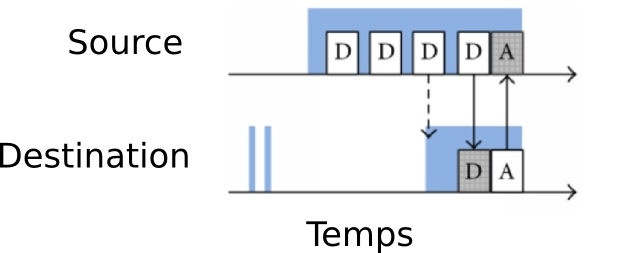
\includegraphics[width=.5\textwidth]{img/contikimac.png}
  \caption{Fonctionnement des réceptions avec ContikiMAC}
  \label{supervision:fig:contikimac}
\end{figure}

La Figure~\ref{supervision:fig:contikimac} illustre le fonctionnement de ContikiMAC.
Pour transmettre une trame de donnée (D), un émetteur l'envoie de manière répétée (``packet strobing'' en anglais) tant qu'une trame d'acquittement (A) n'est pas reçue de la part du récepteur.
Un récepteur va se réveiller périodiquement et faire une écoute du canal pour détecter la présence d'une trame (l'écoute du canal est représentée en bleu sur la figure).
Si aucune émission n'est détectée, le récepteur se rendort.
Quand une émission est détectée, le récepteur passe en réception pour recevoir la trame de donnée dans son intégralité puis, quand la trame de donnée est reçue, une trame d'acquittement est envoyée du récepteur vers l'expéditeur.

Dans le cas d'une trame destinée à tous les voisins (broadcast), elle est répétée sur toute la phase d'activité afin de s’assurer que tous les voisins l’ont reçue au moins une fois.
D'autre part, les voisins n'envoient pas un acquittement à la réception d'une trame envoyée en broadcast.

Si une trame est transmise sur le canal pendant la phase de réveil, le récepteur reste réveillé pour la recevoir sinon il se remet à l’état sommeil.
Lorsqu'un nœud reçoit une trame et qu'elle lui est effectivement destinée, il envoie un acquittement.

Pour optimiser sa transmission, le protocole ContikiMAC utilise une technique de verrouillage de phase.
Elle consiste à estimer la date de réveil du prochain saut pour une destination donnée à partir de la date de réception d’acquittement et de retarder le moment d’émission de paquets jusqu’à l’approche de cette date de réveil.
Cette technique peut économiser de l'énergie en réduisant la quantité de strobing nécessaire à l'envoi d'un paquet en ``synchronisant'' envois et phases de réveil.
Cependant, cette technique n'est pas parfaite, car les horloges internes des différents nœuds ne sont pas synchronisées et des décalages peuvent tout de même se produire~\cite{gonizzi2014rawmac}.

Toujours dans l’objectif d’augmenter la durée de la période de sommeil, le protocole ContikiMAC dispose d'un mécanisme de mise en sommeil rapide pouvant distinguer une transmission de paquet du bruit en comparant la période de l’activité à des longueurs types: (supérieure à la longueur maximale d’un paquet, etc.).
Si la période d'activité n'est pas due à une transmission, le nœud se rendort immédiatement.

Ainsi ContikiMAC permet d'économiser de l'énergie par de multiples techniques, mais cette économie se paye par l'envoi répété d'une trame.
Donc, il est nécessaire de comptabiliser ces retransmissions afin d'avoir une mesure implicite pertinente.

Soit $N_{\textrm{sender}}$ (respectivement $N_{\textrm{receiver}}$) le nombre de fois qu'une source (respectivement une destination) va transmettre (respectivement recevoir) un paquet avec ContikiMAC.

Puisque le destinataire se réveille en moyenne au milieu d'une transmission et attend le prochain essai d'envoi pour recevoir la trame complètement et envoyer son acquittement, le nombre de trames reçues par le destinataire peut être estimé à $N_{\textrm{receiver}} = 1.5$.

Estimer $N_{\textrm{sender}}$ est plus difficile, car cette grandeur dépend des conditions réseau (topologie, qualité du lien) et de la taille des trames.
Ainsi il est nécessaire d'avoir une estimation de ce paramètre afin de procéder à une estimation réaliste de l'utilisation de la radio.

L'expérience suivante est réalisée afin d'estimer le nombre moyen d'essais d'envoi d'une trame de donnée qu'un expéditeur va faire avant de recevoir une trame de confirmation.
Deux nœuds utilisant ContikiMAC sont mis à portée de transmission dans un environnement non bruité.
La source envoie en boucle un paquet de taille fixe qui induit de multiples retransmissions, puis elle attend l'acquittement du paquet et comptabilise le nombre d'essais réalisés avant de recevoir un acquittement et cela pour différentes tailles de paquets.
\ieee{} est utilisé comme simple couche liaison avec un entête pour les trames de données aussi réduit que possible (6 octets) les différentes tailles de trames sont obtenues en faisant varier la taille du message applicatif.
Une simulation simule le comportement de ce système pendant 10000 secondes et pour chaque taille de paquet, l'expérience est exécutée 10 fois avec une graine de générateur de nombre aléatoire différente à chaque fois.

\begin{figure}[h]
  \centering
  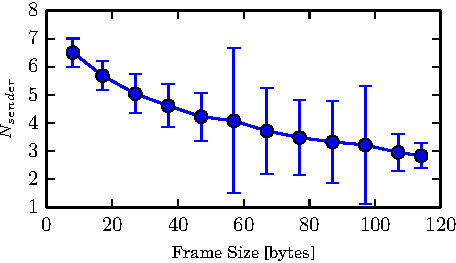
\includegraphics[width=.5\textwidth]{img/average_strobbing-crop.pdf}
  \caption{Nombre moyen de tentatives d'envois en fonction de la taille de la trame avec ContikiMAC.}
  \label{supervision:fig:average_strobing}
\end{figure}

La Figure~\ref{supervision:fig:average_strobing} représente la moyenne du nombre de transmissions $N_{\textrm{sender}}(f)$ nécessaires à l'envoi d'une trame $f$ ayant une taille de $\mathcal{L}(f)$ octets entre deux nœuds fonctionnant avec ContikiMAC.
Le nombre d'envois moyens nécessaires pour envoyer un long paquet est plus faible que pour en envoyer un court, car les trames longues mettent plus de temps pour être transmises et ont donc plus de chance d'être écoutées pendant un réveil du destinataire.
% En outre, comme les paquets \ac{ACK} ont une taille constante, le coût de réception pour la source est constant.
% Cette valeur est inférieure à celle de $N_{\textrm{receiver}}$ ainsi c'est donc l'expéditeur qui va dépenser le plus d'énergie quand ContikiMAC est employé.

On peut remarquer que la variance est également faible pour des trames de grande taille ce qui est également cohérent, car le nombre d'envois qu'il est possible de faire pour une trame de cette taille au cours d'un cycle complet est limité ainsi la variance est réduite. 

\section{Validation expérimentale}
\label{supervision:validation}

\subsection{Supervision passive}
\label{supervision:chain_results}

\begin{figure}[ht]
  \centering
  \begin{tikzpicture}

  % définition des styles
  \tikzstyle{child}=[circle, draw, fill=yellow!50,text=black]
  \tikzstyle{router}=[circle, draw, fill=orange!50,text=black]
  \tikzstyle{root}=[circle, draw, fill=red!50,text=black]

  % Réseau contraint
  \node[root] (root) {G};
  \node[router, left=of root] (1) {1};
  \node[router, left=of 1] (2) {2};
  \node[router, left=of 2] (3)  {3};
  \node[router, left=of 3] (4) {4};
  \node[router, left=of 4] (5) {5};
  \node[child, left=of 5] (6) {6};

\path

  (6.east) edge[->, thin] (5.west)
  (5.east) edge[->, thin] (4.west)
  (4.east) edge[->, semithick] (3.west)
  (3.east) edge[->, thick] (2.west)
  (2.east) edge[->, very thick] (1.west)
  (1.east) edge[->, ultra thick] (root.west)
  ;

  \end{tikzpicture}

  \caption{Topologie réseau utilisée pour mesurer la précision de la mesure implicite et passive}

  \label{supervision:fig:topology_chain}
\end{figure}

Une topologie chaînée à 7 nœuds comme représentée sur la Figure~\ref{supervision:fig:topology_chain} est utilisée pour tester le mécanisme décrit ci-dessus.
Dans cette configuration, les nœuds ne peuvent envoyer et recevoir de  paquets que de la part de leurs voisins adjacents.
Tous les paquets remontent vers la passerelle représentée par un G sur la figure.

Les nœuds utilisent le système Contiki~\cite{dunkels2004contiki}, \ieee{} pour communiquer et ContikiMAC comme mécanisme de cycle de veille.
\ac{RPL}~\cite{rfc6550} est le protocole de routage utilisé et il est configuré en non-storing mode, c'est-à-dire qu'il a accès à toute la topologie réseau et en particulier aux routes descendantes.

Durant 200 secondes, chaque nœud envoie au \ac{LBR} un paquet \ac{UDP} à chaque seconde avec une charge utile de 10 octets ce qui induit une trame de 69 octets chaque seconde.
Le trafic applicatif d'un nœud démarre lorsqu'il joint la topologie réseau, il a alors un parent qui est son voisin adjacent.

D'après les résultats expérimentaux (Figure. \ref{supervision:fig:average_strobing}), l'utilisation de ContikiMAC induit qu'une trame de 69 octets est émise en moyenne 3,76 fois avant d'être reçue.
Le mécanisme de mesure implicite tient compte de ce phénomène et l'applique à chaque routeur intermédiaire afin que l'utilisation de la radio soit en accord avec ce résultat.

Les temps de transmission et de réception des nœuds sont obtenus par l'utilisation du simulateur et de Powertracker~\cite{dunkels2011powertrace} qui permet d'obtenir le temps passé dans chaque état de transmission radio pour chaque nœud avec une résolution de $1 \mu s$.
Puisque la passerelle est toujours éveillée, elle reçoit donc du premier coup toutes les trames: $N_{\textrm{receiver}} = 1$.

\subsubsection{Analyse de l'impact de la profondeur}
\label{supervision:depth_analysis}

\begin{figure}[ht]
  \begin{subfigure}{0.5\textwidth}
    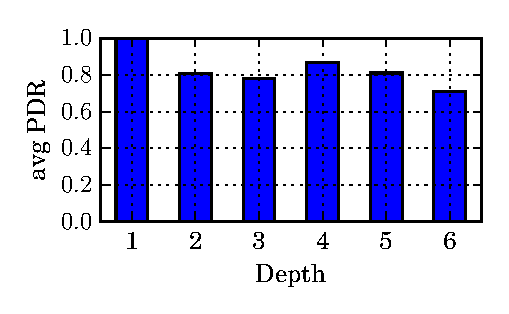
\includegraphics[width=\textwidth]{img/pdr_depth.pdf}
    \caption{Packet Delivery Ratio (PDR).}
    \label{supervision:fig:pdr_depth}
  \end{subfigure}
  \begin{subfigure}{0.5\textwidth}
    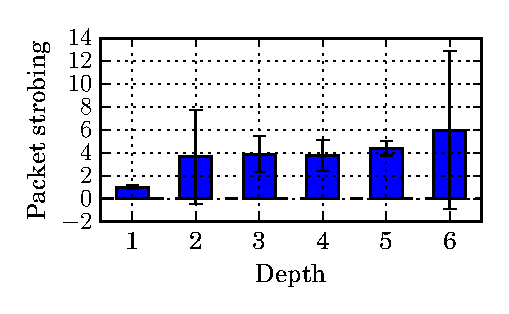
\includegraphics[width=\textwidth]{img/strobes_depth.pdf}
    \caption{Tentatives d'envois de paquets par profondeur.}
    \label{supervision:fig:strobes_depth}
  \end{subfigure}
  \caption{Impact de la profondeur}
\end{figure}

\paragraph{\ac{PDR}}

La figure Fig.~\ref{supervision:fig:pdr_depth} représente le ratio de succès de transmission de paquets applicatifs pour chaque nœud en fonction de la distance à la racine en nombre de sauts.
Cette figure montre la proportion du trafic applicatif que la passerelle peut effectivement voir.
Le ratio de paquets acheminés n'est pas uniforme sur tout le \ac{LLN} et les nœuds qui ne sont pas connectés directement à une racine souffrent de pertes de paquets non négligeables malgré un trafic faible en raison d'un grand nombre de retransmissions de paquets.

Le routeur de bordure n'utilise pas ContikiMAC car dans les hypothèses de l'expérience, il n'est pas contraint en énergie et peut donc rester éveillé en permanence.
Ainsi, tous les paquets issus du nœud 1 sont reçus prouvant que ContikiMAC induit des pertes et nuit à la fiabilité des transmissions pour les nœuds plus éloignés.

Puisqu'un paquet peut être perdu à chaque fois qu'il traverse un routeur fonctionnant avec ContikiMAC, traverser de nombreux routeurs augmente la probabilité que les paquets soient perdus, car \ac{UDP} ne fournit aucun mécanisme de fiabilité.
Ce phénomène est confirmé par la Figure~\ref{supervision:fig:pdr_depth} où la quantité de paquets arrivant à la racine semble décroître globalement à mesure qu'on s'en éloigne.

\paragraph{Retransmissions de paquets (``Packet strobing'')}

La Figure~\ref{supervision:fig:strobes_depth} représente le nombre moyen d'envois de paquets i.e. le nombre de tentatives que va faire chaque nœud pour envoyer une trame à son parent.

Les valeurs obtenues précédemment restent expérimentalement proches de la valeur de 3,76 obtenue expérimentalement (Figure \ref{supervision:fig:average_strobing}).
Cependant, la variance est forte et le nombre de tentatives tend à augmenter à mesure que l'on s'éloigne de la racine.
Cette variance peut être expliquée par la variance obtenue pour des trames de 69 octets sur l'expérience de calcul des $N_{sender}$.

La convergence vers la valeur normale de 3,76 pour les nœuds proches de la racine s'explique par l'augmentation du trafic réseau sur ces nœuds: ils doivent relayer les paquets provenant de tous les autres nœuds.
Ainsi, leur rythme d'envoi se rapproche de celui de l'expérience de strobing où la source envoyait autant de paquets que possible vers un destinataire en s'assurant de son acquittement.
Pour un nœud situé en bout de chaîne et n'ayant donc aucune charge de routage, un plus grand décalage entre les cycles d'éveils est présent et explique ainsi les retransmissions supplémentaires.

Enfin, au sujet du nœud qui est connecté à la passerelle directement, la quantité moyenne d'envois est très proche de 1 avec une variance faible, ce qui est logique puisque par hypothèse la racine est toujours éveillée et peut donc recevoir immédiatement les transmissions qui en viennent.
Cependant, ce n'est pas le cas des nœuds se situant juste avant le nœud 1, qui reçoivent une quantité importante de trafic, mais qui ne peuvent pas la router avec la même efficacité (temporisation, ``buffering'', etc.).

\subsubsection{Analyse de l'impact des protocoles}
\label{supervision:protocols_analysis}

Connaître la répartition des protocoles au cours du temps permet de savoir la proportion de ressources investies dans le maintien du réseau et celle investie dans un but applicatif à valeur ajoutée.

\begin{figure}[ht]
  \begin{subfigure}{0.5\textwidth}
    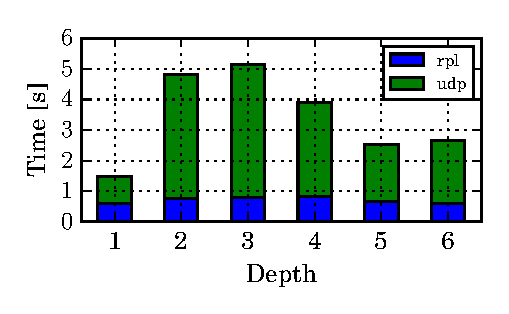
\includegraphics[width=\textwidth]{img/protocol_repartition_depth.pdf}
    \caption{Répartition des protocoles par profondeur.}
    \label{supervision:fig:protocol_repartition}
  \end{subfigure}
  \begin{subfigure}{0.5\textwidth}
    \centering
    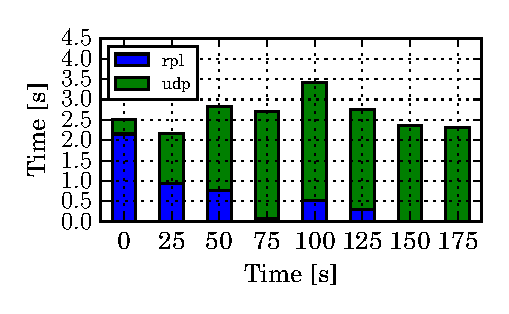
\includegraphics[width=\textwidth]{img/repartition_protocol.pdf}
    \caption{Évolution de la répartition des protocoles (statistiques par fenêtres de 25 secondes.}
    \label{supervision:fig:protocol_repartition_time}
  \end{subfigure}%
  \caption{Impact des protocoles}
\end{figure}

\paragraph{Répartition des protocoles}

La Figure~\ref{supervision:fig:protocol_repartition} met en évidence que la quantité de trafic lié au protocole de routage est relativement homogène pour tous les nœuds.
Ce phénomène est lié à la topologie et au fonctionnement de \ac{RPL}: les nœuds n'envoient de paquets de routage qu'à un seul parent à la fois ainsi le trafic de routage est le même pour tous les nœuds du réseau.

\paragraph{Évolution au cours du temps}

La Figure~\ref{supervision:fig:protocol_repartition_time} met en évidence l'évolution typique de la répartition des protocoles au cours du temps.
La charge liée au protocole de routage est très importante lors du démarrage du réseau, car aucune route n'est alors disponible.
Ainsi l'essentiel du trafic observé correspond à des paquets \ac{RPL} qui sont utilisés pour mettre à jour les routes sur chaque nœud.

\ac{RPL} étant proactif, les routes sont construites et entretenues en permanence, ainsi même après la construction de la topologie, du trafic \ac{RPL} est toujours émis.
Cependant, le mécanisme de ``Trickle'' réduit la quantité de paquets émis pour maintenir la topologie qui est observée.

Cette évolution du trafic permet de déduire qu'un mécanisme n'ayant pas la connaissance des routes manquerait non seulement l'impact du relayage sur les routeurs dans la topologie, mais aussi la charge impliquée par la construction des routes qui est non négligeable même dans le cas d'une topologie simple comme celle d'une chaîne.

Cependant, le trafic applicatif est majoritaire lorsque le réseau est stable, ainsi l'approche par supervision passive peut être explorée, car l'essentiel du trafic a vocation à passer par le routeur de bordure.

\subsection{Précision de la mesure passive de l'utilisation de la radio}

Le mécanisme d'estimation se déclenche quand toutes les routes sont établies et qu'un trafic réseau est observé à la passerelle.
L'estimation du temps radio va alors fournir une estimation pour le temps passé en transmission et en réception pour chaque nœud.

On appelle \emph{précision} $\delta = \frac{\widehat{X}}{X}$ le rapport entre l'estimation d'une grandeur $\widehat{X}$ et sa valeur réelle $X$ qui est mesurée dans le simulateur.
Cette métrique permet d'interpréter facilement les grandeurs trouvées: $\delta \leq 1$ (respectivement $\delta \geq 1$) signifie que l'estimation sous-estime (respectivement surestime) la grandeur.
Cette section mesure la précision des estimations passives pour les cas d'estimation ``étoilée'' (où la topologie de routage est inconnue) et ``maillée'' (où la topologie de routage est connue).

\subsubsection{Précision en fonction de la topologie}

\begin{figure}[ht]
  \begin{subfigure}{0.5\textwidth}
    \centering
    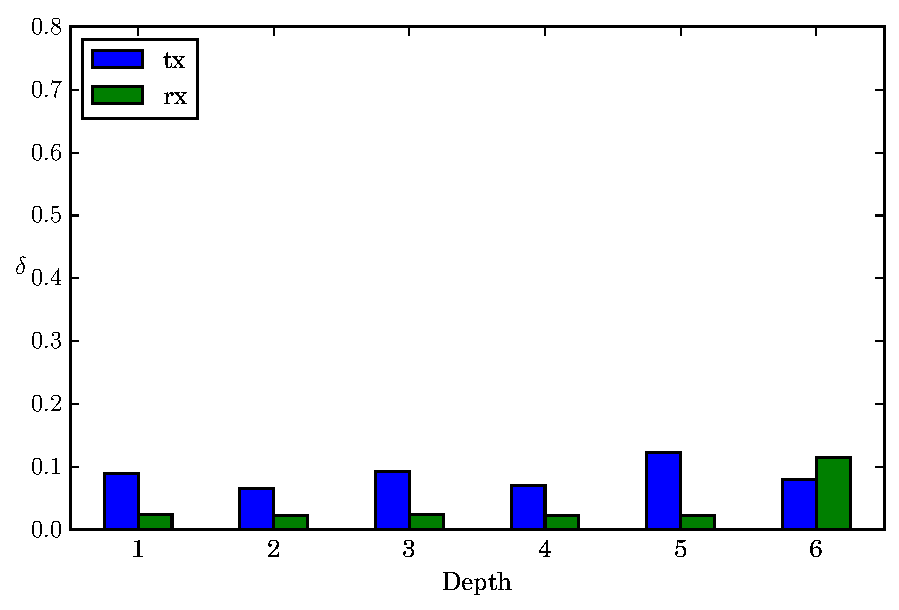
\includegraphics[width=\textwidth]{img/global_noinfo.pdf}
    \caption{$\delta$ total global pour l'estimation ``étoilée''}
    \label{supervision:fig:global_noinfo}
  \end{subfigure}
  \begin{subfigure}{0.5\textwidth}
    \centering
    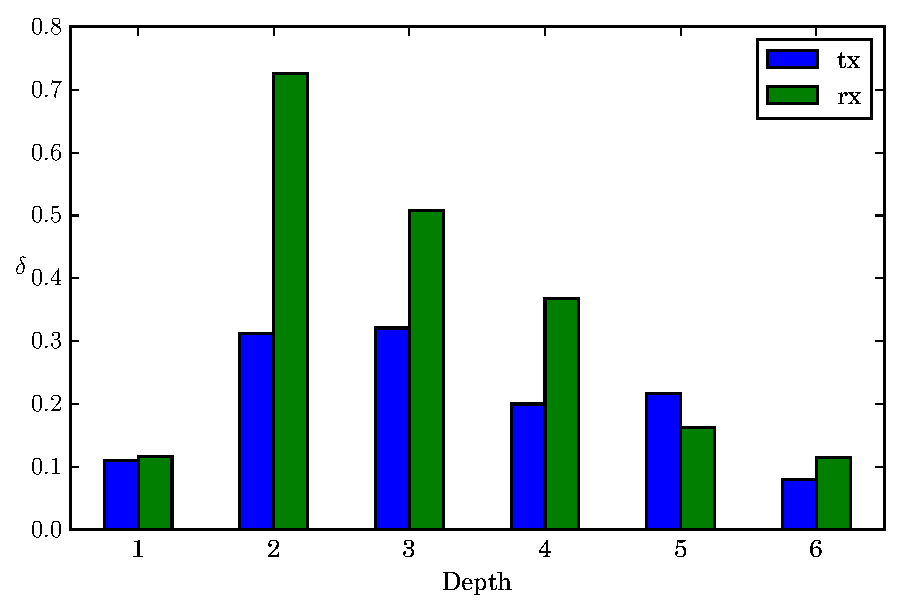
\includegraphics[width=\textwidth]{img/global_route.pdf}
    \caption{$\delta$ total global pour l'estimation ``maillée''}
    \label{supervision:fig:global_route}
  \end{subfigure}
  \caption{$\delta$ total et global par profondeur}
  \label{supervision:fig:global}
\end{figure}

La Figure~\ref{supervision:fig:global} montre que la précision obtenue à la fin de la simulation pour chaque nœud est sous-estimée.
Ce phénomène est attendu, car la mesure implicite ne peut inférer tous les phénomènes, de plus l'approche proposée n'introduit pas de mécanismes ad hoc pour augmenter les estimations.

Dans le cas de l'estimation ``étoilée'', $\delta$ est homogène pour l'ensemble des nœuds qui ont pour charge de router des paquets qui ne leur sont pas destinés comme le montre la Figure~\ref{supervision:fig:global_noinfo}.
C'est cohérent avec la nature de l'estimation ``étoilée'' qui ne prend pas en compte toute la charge liée au routage.
De plus, la réception est plus sous-évaluée que la transmission, car elle ne prend en compte que la réception des trames d'acquittement qui représentent un volume très restreint sauf pour le nœud 6 qui n'a pas d'autre charge de réception.

Dans le cas de l'estimation ``maillée'', $\delta$ est plus élevé, car l'utilisation de la radio liée aux retransmissions est prise en charge ainsi une plus grande part du trafic est déduite des observations passives.
On remarque un net progrès pour la réception qui d'une part est régulière à prévoir avec ContikiMAC ($N_{receiver} = 1.5$) et d'autre part parce que le volume de routage est plus important.

Les erreurs d'estimations restent cependant importantes, car dans les deux cas, une part importante du trafic n'est pas inféré (pertes de paquets, variance du strobbing, trafic de routage local non transmis à la passerelle, etc.).

En outre, la mesure implicite ``étoilée'' ou ``maillée'' est identique pour le nœud feuille par construction, car aucune charge de routage ne lui est appliqué dans les deux cas.

\subsubsection{Évolution de $\delta$ au cours du temps}

Cette section étudie l'évolution de $\delta$ au cours du temps afin d'affiner la compréhension des facteurs pouvant expliquer la sous-estimation obtenue dans la section précédente.
Les résultats suivants sont obtenus en découpant l'expérience sur des intervalles de 20 secondes.
$\delta$ est alors le temps de radio estimé sur le temps réel dans cet intervalle uniquement.

\paragraph{Estimation ``étoilée''}

\begin{figure}[h]
  \centering
  \begin{subfigure}{0.3\textwidth}
    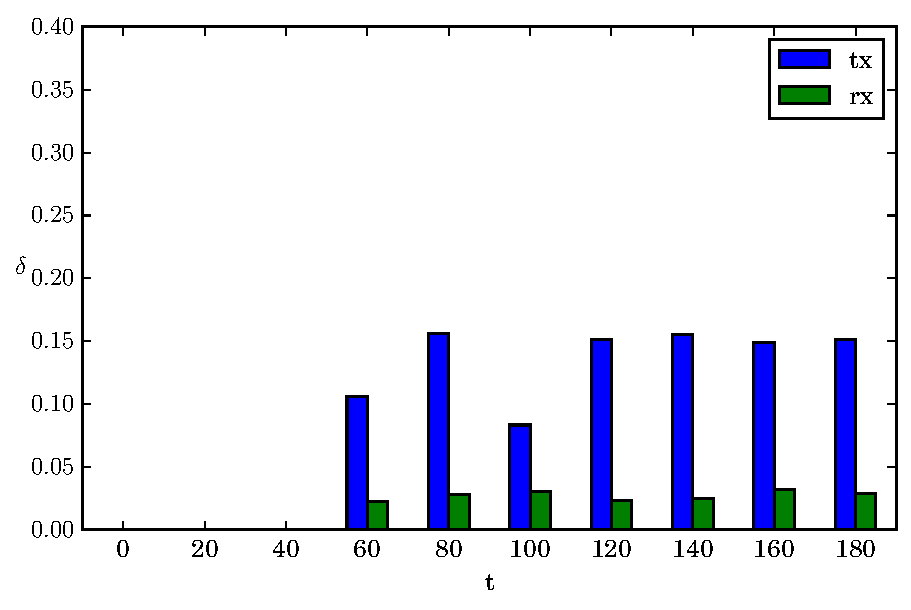
\includegraphics[width=\textwidth]{img/evolution_noinfo_1.pdf}
    \caption{Profondeur: 1}
    \label{supervision:fig:noinfo_1}
  \end{subfigure}
  \begin{subfigure}{0.3\textwidth}
    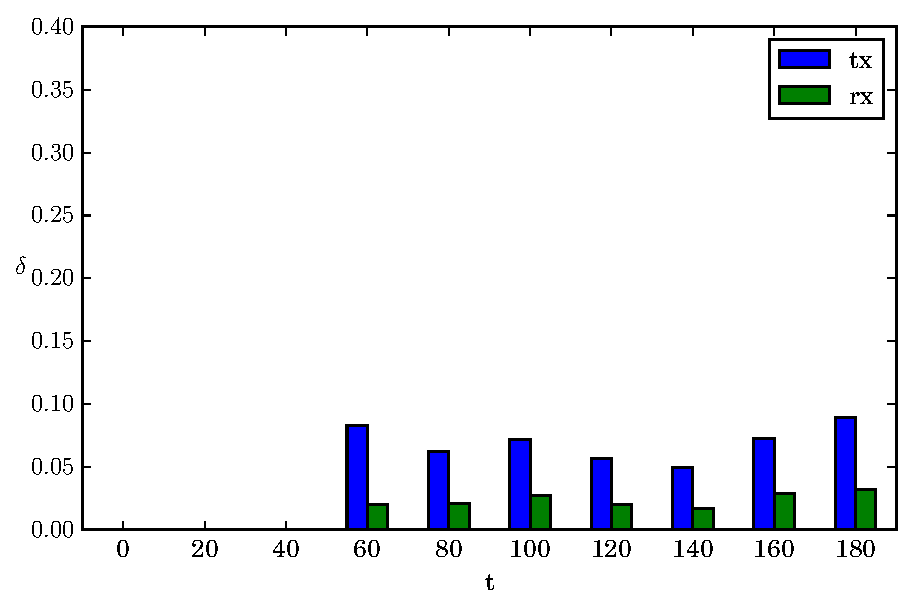
\includegraphics[width=\textwidth]{img/evolution_noinfo_2.pdf}
    \caption{Profondeur: 2}
    \label{supervision:fig:noinfo_2}
  \end{subfigure}
  \begin{subfigure}{0.3\textwidth}
    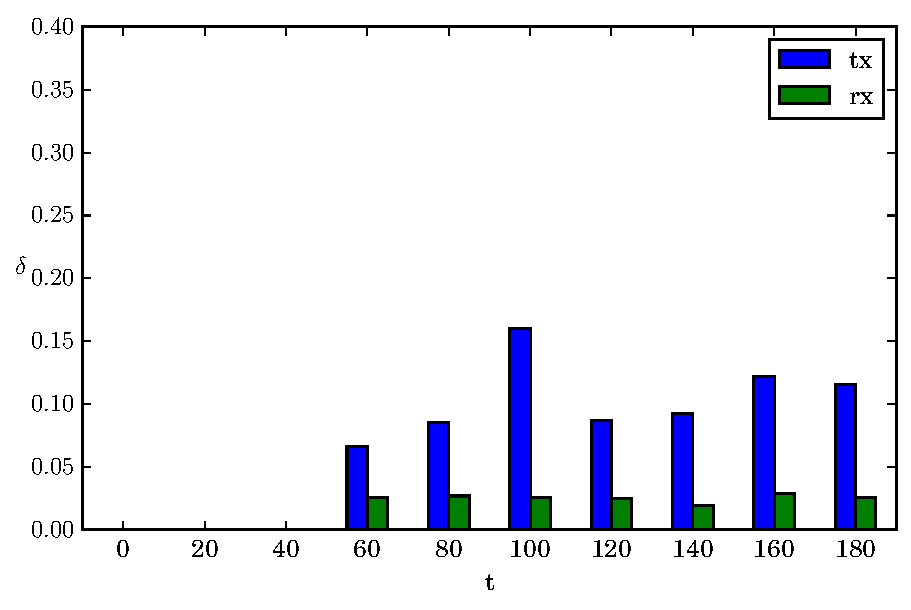
\includegraphics[width=\textwidth]{img/evolution_noinfo_3.pdf}
    \caption{Profondeur: 3}
    \label{supervision:fig:noinfo_3}
  \end{subfigure}

  \begin{subfigure}{0.3\textwidth}
    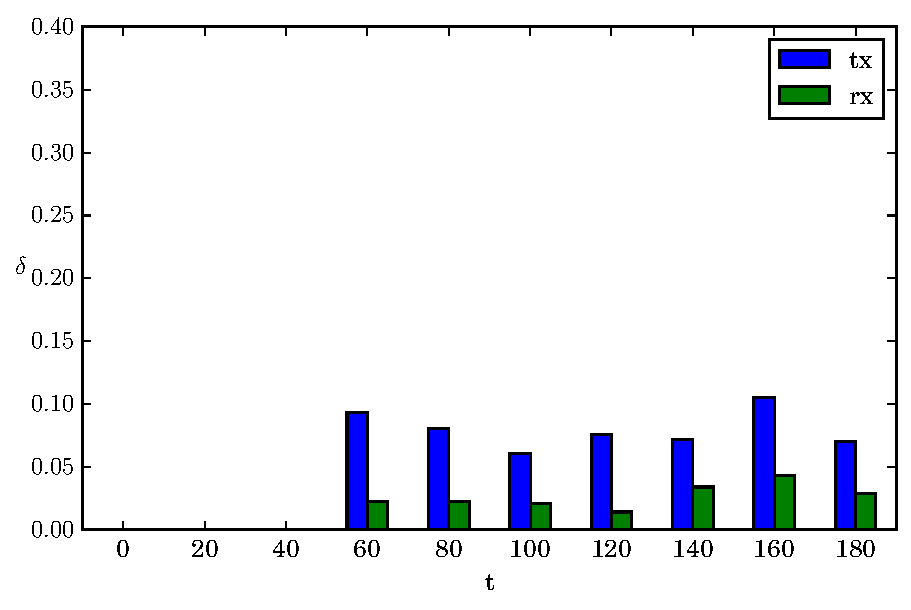
\includegraphics[width=\textwidth]{img/evolution_noinfo_4.pdf}
    \caption{Profondeur: 4}
    \label{supervision:fig:noinfo_4}
  \end{subfigure}
  \begin{subfigure}{0.3\textwidth}
    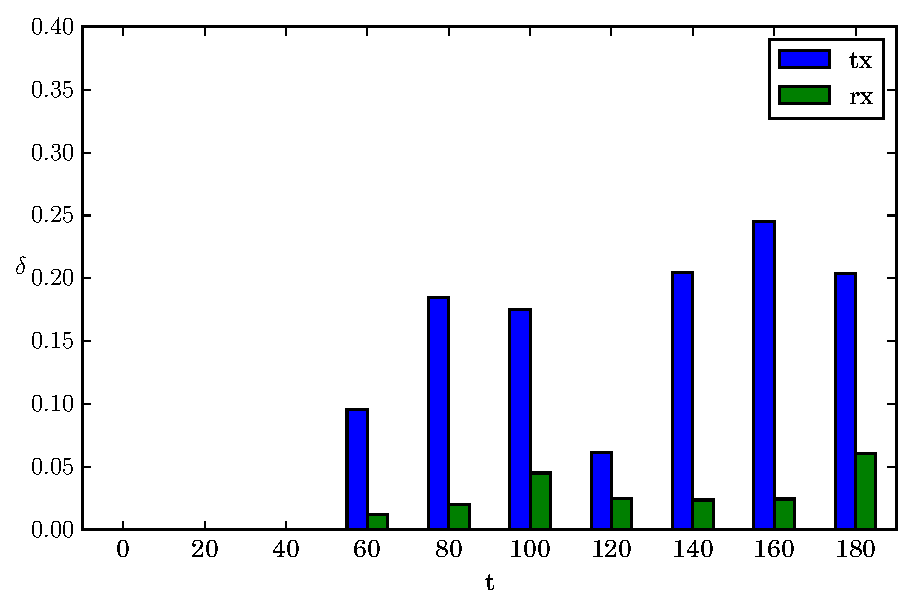
\includegraphics[width=\textwidth]{img/evolution_noinfo_5.pdf}
    \caption{Profondeur: 5}
    \label{supervision:fig:noinfo_5}
  \end{subfigure}
  \begin{subfigure}{0.3\textwidth}
    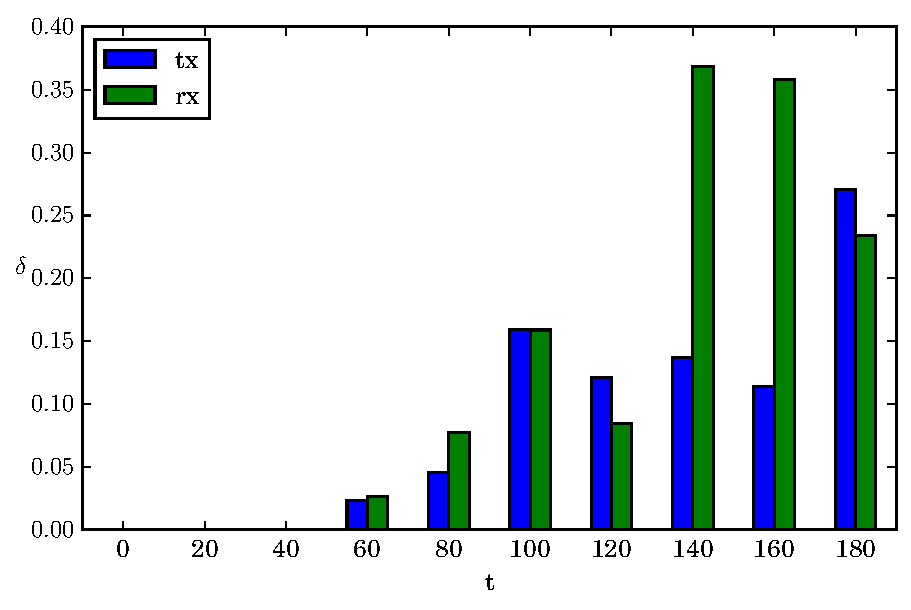
\includegraphics[width=\textwidth]{img/evolution_noinfo_6.pdf}
    \caption{Profondeur: 6}
    \label{supervision:fig:noinfo_6}
  \end{subfigure}
  \caption{Évolution de $\delta$ pour une estimation ``étoilée''}
  \label{supervision:fig:noinfo}
\end{figure}

La Figure~\ref{supervision:fig:noinfo} détaille pour chaque nœud l'évolution de $\delta$ pour une estimation ``étoilée''.
La sous-estimation continue, car les processus non visible depuis la passerelle (routage des paquets, pertes de paquets, etc.) continuent au cours de l'expérience.

Les nœuds situés à une plus grande profondeur relaient moins de paquets ainsi leur $\delta$ augmente, car une plus grande proportion de leur trafic applicatif est connue par le routeur de bordure au fur et à mesure de l'expérience.
D'autre part, $\delta$ augmente au cours du temps, car le trafic applicatif qui est celui inféré par la mesure passive prend une part plus importante au cours du temps (\ref{supervision:fig:protocol_repartition_time}).

\paragraph{Estimation ``maillée''}

\begin{figure}[h]
  \centering
  \begin{subfigure}{0.3\textwidth}
    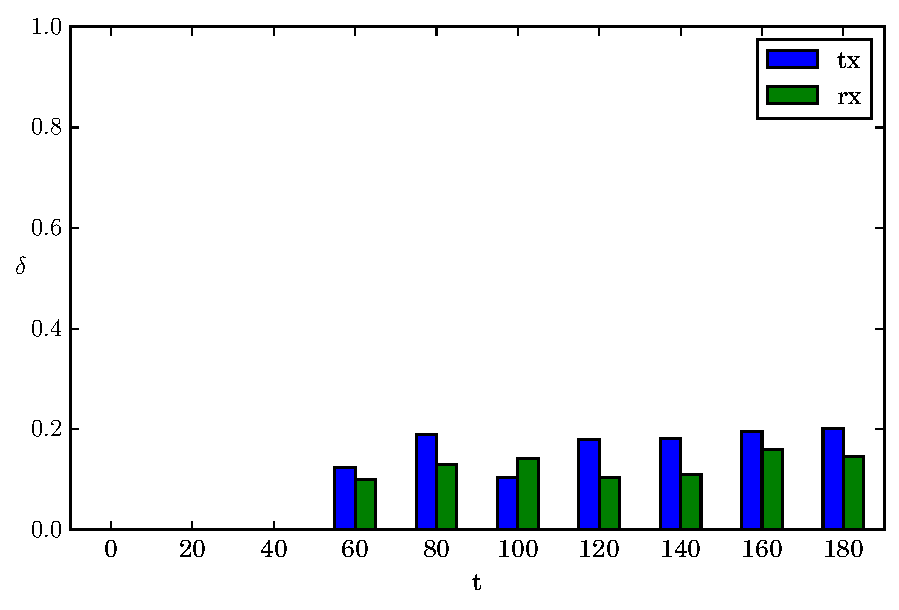
\includegraphics[width=\textwidth]{img/evolution_route_1.pdf}
    \caption{Profondeur: 1}
    \label{supervision:fig:route_1}
  \end{subfigure}
  \begin{subfigure}{0.3\textwidth}
    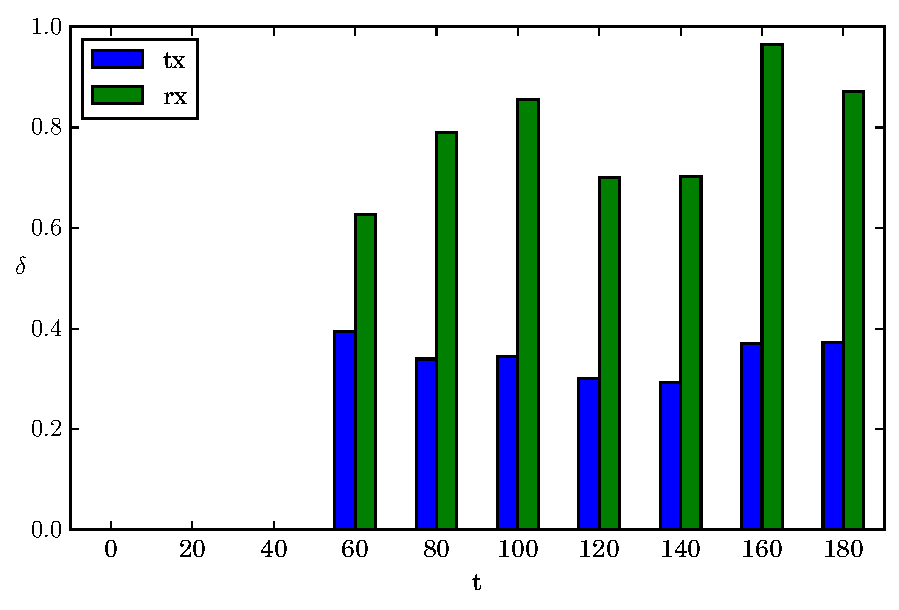
\includegraphics[width=\textwidth]{img/evolution_route_2.pdf}
    \caption{Profondeur: 2}
    \label{supervision:fig:route_2}
  \end{subfigure}
  \begin{subfigure}{0.3\textwidth}
    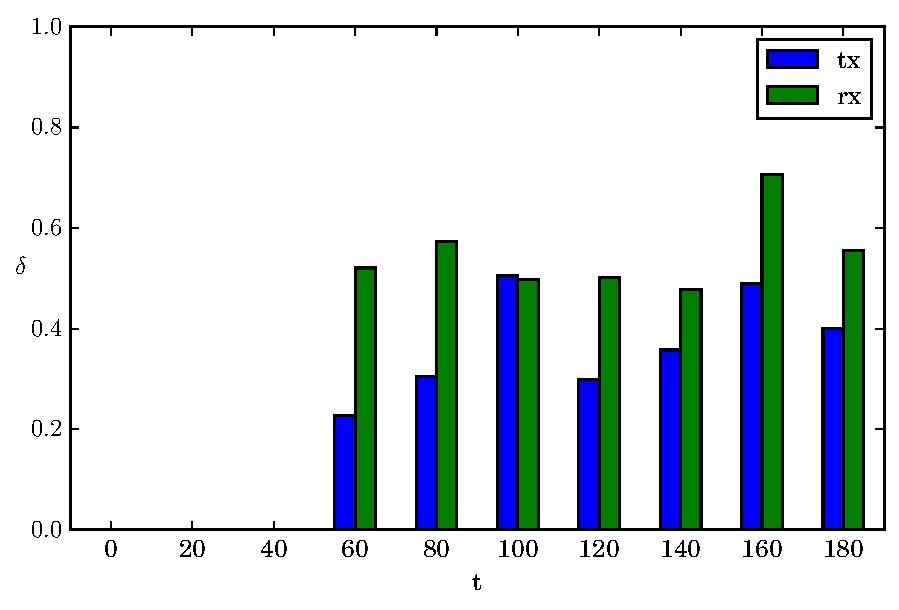
\includegraphics[width=\textwidth]{img/evolution_route_3.pdf}
    \caption{Profondeur: 3}
    \label{supervision:fig:route_3}
  \end{subfigure}

  \begin{subfigure}{0.3\textwidth}
    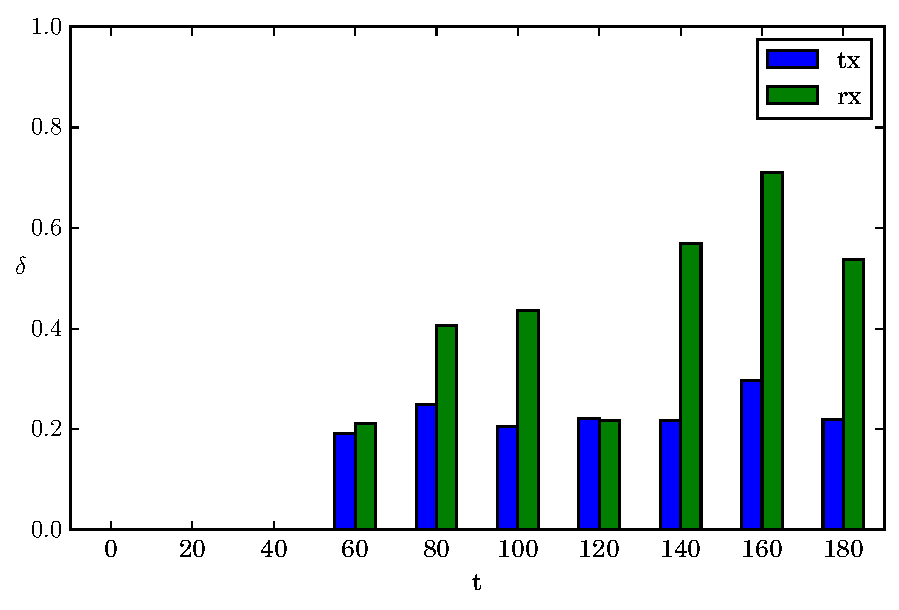
\includegraphics[width=\textwidth]{img/evolution_route_4.pdf}
    \caption{Profondeur: 4}
    \label{supervision:fig:route_4}
  \end{subfigure}
  \begin{subfigure}{0.3\textwidth}
    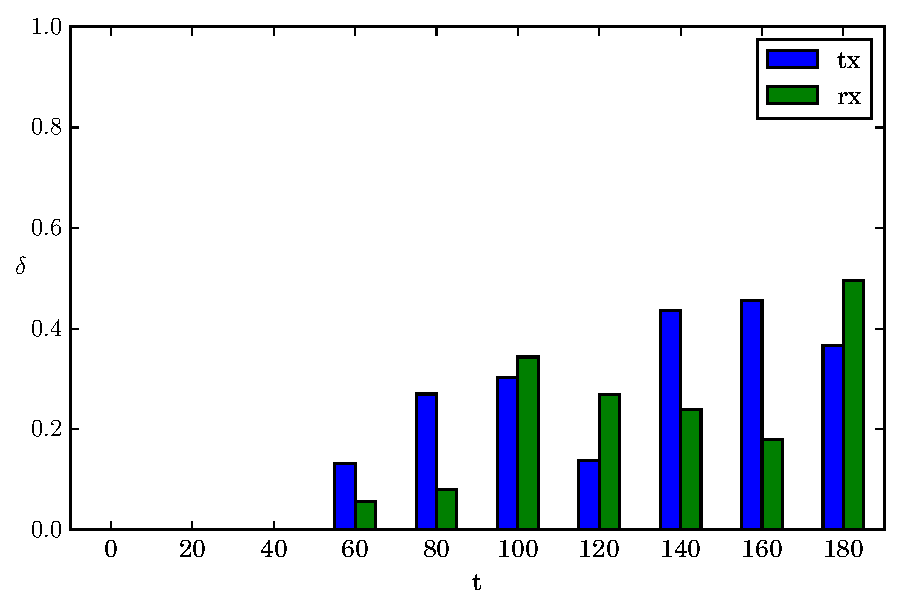
\includegraphics[width=\textwidth]{img/evolution_route_5.pdf}
    \caption{Profondeur: 5}
    \label{supervision:fig:route_5}
  \end{subfigure}
  \begin{subfigure}{0.3\textwidth}
    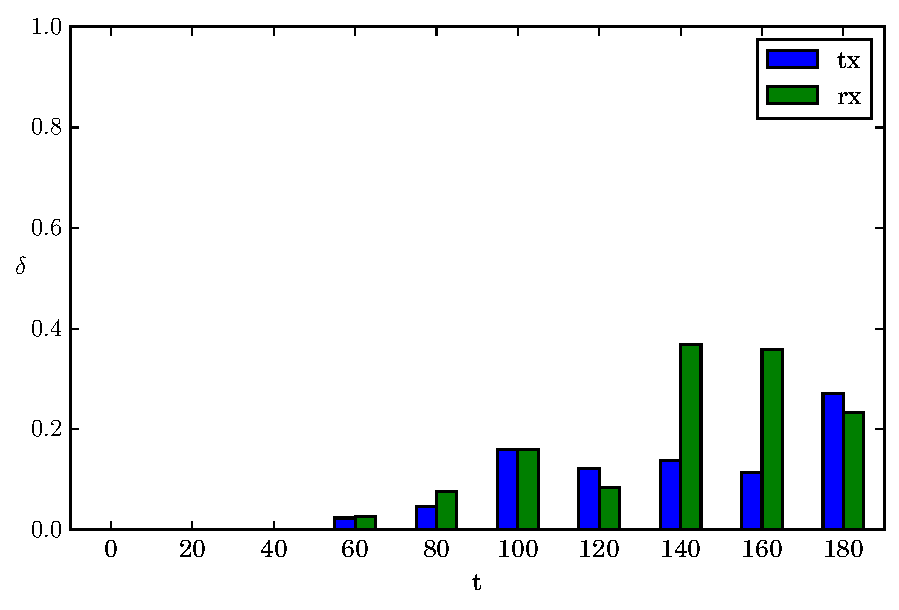
\includegraphics[width=\textwidth]{img/evolution_route_6.pdf}
    \caption{Profondeur: 6}
    \label{supervision:fig:route_6}
  \end{subfigure}
  \caption{Évolution de l'$\delta$ pour une estimation ``maillée''}
  \label{supervision:fig:route}
\end{figure}

L'estimation maillée est meilleure sur tous les intervalles de temps, ce qui est attendu, car elle comptabilise la charge de routage sur chacun de ces intervalles en plus de l'estimation étoilée.

D'autre part, l'estimation s'améliore au cours du temps, car non seulement le trafic applicatif devient majoritaire au cours du temps comme montré sur la Figure~\ref{supervision:fig:protocol_repartition_time} mais en plus la charge de routage intermédiaire qu'il induit est également comptabilisée.

% Discussion

Cependant, l'erreur d'estimation est encore forte en raison des pertes de paquets et des variations de la quantité de ``strobbing'' nécessaire pour transmettre un paquet à chaque saut.
Ainsi si la quantité de strobbing est sous-estimée, sur chaque saut l'impact de chaque paquet sur l'estimation de la radio est grandement perturbé.

Afin de limiter le strobbing, une solution serait d'avoir des trames aussi remplies que possible (par exemple avec des informations au sujet des nœuds.).
Ainsi, la quantité de strobbing nécessaire serait beaucoup plus faible, car les trames seraient détectées au bout d'un faible nombre de tentatives.

Une autre solution possible consiste à envoyer à intervalles réguliers des informations de ``recalibrations'' afin de recaler les estimations pour fournir des valeurs correctes.

\section{Mesures explicites}
\label{supervision:explicite}

La passerelle peut effectuer une mesure passive du temps passé par les nœuds du \ac{LLN} en transmission et en réception.
Cependant, les paquets perdus, retransmis ou non routés vers la passerelle ne sont pas comptabilisés avec cette méthode qui induit donc un biais.

Ainsi des mécanismes de mesure active semblent inévitables pour obtenir une information fiable.
Ces messages peuvent être envoyés à la passerelle par ``piggybacking'' ou être mis dans les paquets du protocole de routage utilisé.

Cependant, le rythme de ces mesures doit être modéré afin de limiter la consommation de ressources qu'il induit.
Ainsi si les temps entre deux envois de mesures explicites sont longs, la mesure implicite de la radio précédemment introduite peut fournir une approximation entre ces deux envois.

Quand la passerelle reçoit une mesure explicite au temps $t$ elle recalcule son estimation pour la grandeur $\widehat{X}$ de la manière suivante:

\begin{align}
  \widehat{X}(t) &= X(t_r) + \epsilon(t_r)\frac{t - t_r}{T}\\
  \epsilon(t_r) &= \alpha (X(t_r) - \widehat{X}(t_r)) + (1 - \alpha)\epsilon(t_{r-1})
  \label{supervision:eqn:bias}
\end{align}

où $t_r$ et $t_{r-1}$ sont les deux dernières dates de réception de mesure active.
$T$ désigne le temps entre chaque mesure explicite reçue.
$X(t_r)$ désigne la valeur obtenue par mesure explicite à l'instant $t_r$.
$\epsilon(t_r)$ est l’estimation de l'erreur apprise des précédents messages de mesure active~\footnote{Par convention: $\epsilon(0) = 0$}.
Cette erreur est calculée par une \ac{EWMA} de paramètre $\alpha$~\cite{mckinney2012python}.
Le coefficient $\alpha$ compris entre 0 et 1 représente le degré de décroissance des erreurs des valeurs passées.
Une valeur de $\alpha$ importante réduira plus rapidement l'importance des observations passées.
A un instant $t$, l'erreur est prise proportionnellement au temps depuis la dernière mesure explicite reçue.


% $\frac{X(t_r) - X(t_{r-1})}{t_r - t_{r-1}}$ représente la tendance de la grandeur $X$. 
% Le paramètre $\alpha$ désigne la proportion de l'estimation 

\subsection{Validation expérimentale}

\begin{figure}[ht]
  \centering
  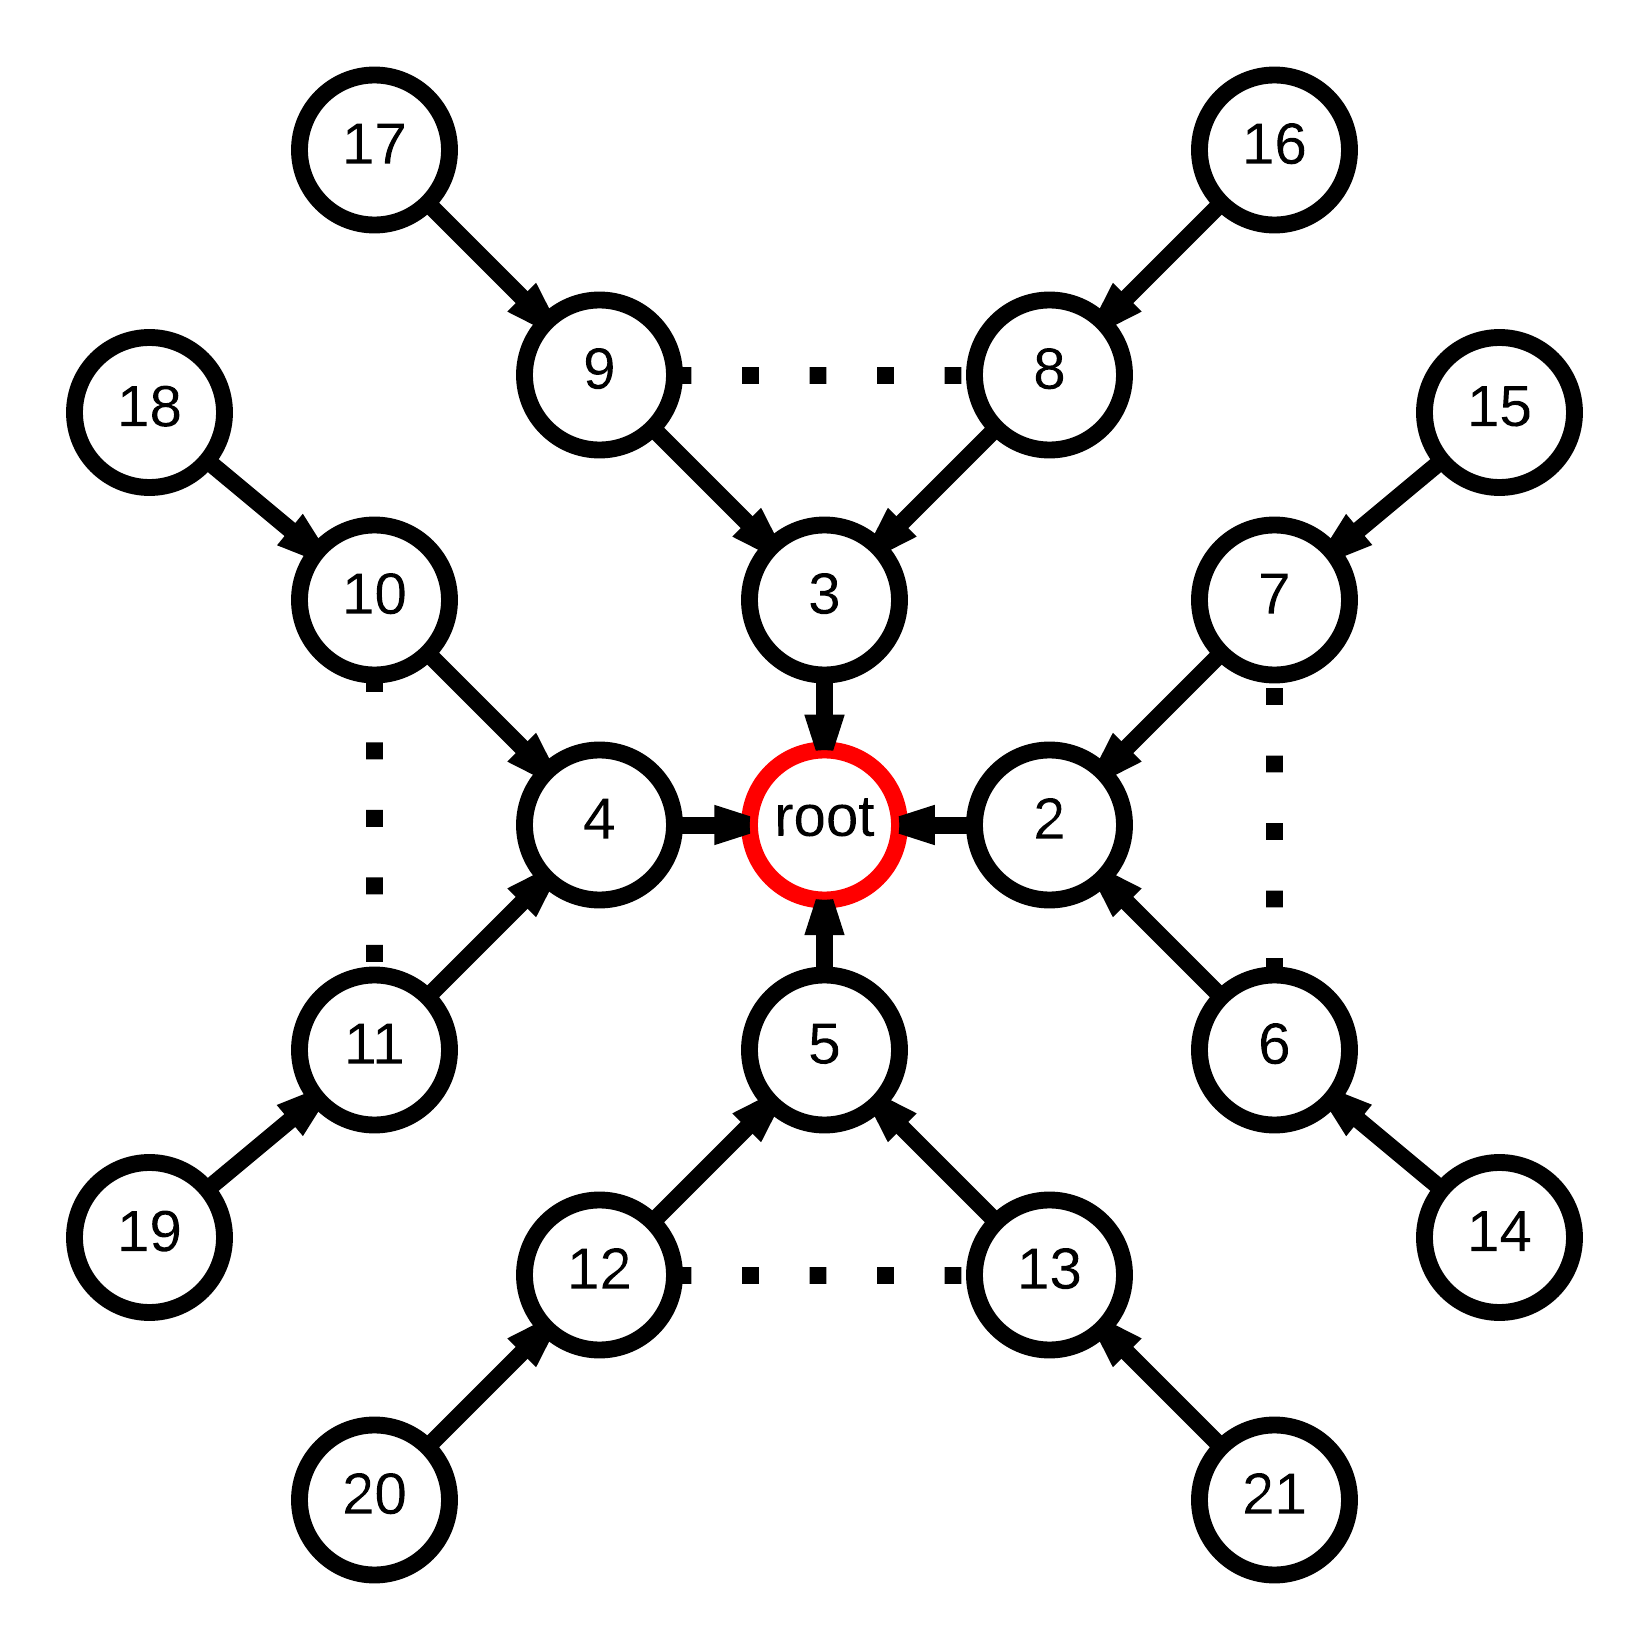
\includegraphics[width=0.5\textwidth]{img/topology_tree.png}
  \caption{Topologie réseau et radio.}
  \label{supervision:fig:topology_tree}
\end{figure}

Cette méthode de recalibration des mesures passives est évaluée en utilisant une topologie représentée sur la Figure~\ref{supervision:fig:topology_tree} composée de 21 nœuds envoyant des paquets applicatifs à la racine chaque seconde pendant 200 secondes.
Les messages contenant des mesures exactes des temps mesurés par le nœud passé dans chaque état de transmission sont envoyés par les nœuds par un mécanisme de publish-subscribe pour économiser le coût d'une requête.
La fréquence de ces envois de recalibrations est réglée par l'administrateur.

Comme vu dans les validations précédentes, le réseau est peu régulier et les phénomènes de strobing ont une grande variance.
Ainsi, afin de ne pas réagir trop brutalement aux changements d'une mesure et de privilégier les tendances de fond, le paramètre de décroissance de l'\ac{EWMA} est mis à $\alpha = 0.25$.

\paragraph{Erreur relative globale}

\begin{figure}[ht]
  \centering
  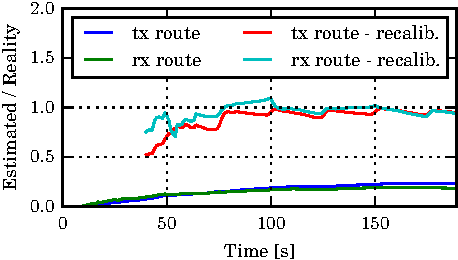
\includegraphics{img/ratio_recalibration_global-crop.pdf}
  \caption{Erreur d'estimation globale pour une topologie en arbre avec et sans recalibration dynamique (toutes les 25 secondes).}
  \label{supervision:fig:tree_calibration}
\end{figure}

La Figure~\ref{supervision:fig:tree_calibration} montre le rapport entre la valeur estimée et la valeur réelle moyenne quand des messages de supervisions périodiques sont envoyés par les nœuds toutes les 25 secondes.
A chaque mesure explicite, l'estimateur intègre l'erreur moyenne des précédentes mesures et converge ainsi vers une estimation correcte.
On observe également que les pentes des estimations après chaque recalibrations sont moins grandes, car l'estimateur apprend son biais qui est supposé constant pendant l'expérience.
Ainsi on obtient une estimation qui a tout temps est capable de produire une estimation du temps passé en transmission et en réception.

\paragraph{Fréquence de recalibrage}

\begin{figure}[ht]
  \centering
  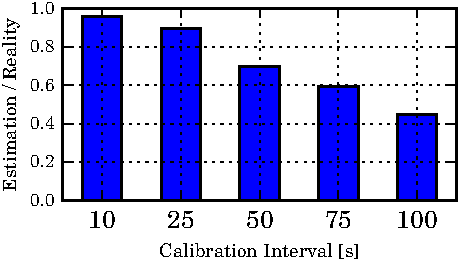
\includegraphics{img/ratio_recalibration-crop.pdf}
  \caption{Erreur relative pour différents intervalles de supervision active.}
  \label{supervision:fig:frequencies_error}
\end{figure}

La Figure~\ref{supervision:fig:frequencies_error} montre l'erreur moyenne globale obtenue par le mécanisme avec une estimation étoilée en fonction des périodes entre chaque message de supervision active.
Sur une expérience durant 200 secondes, n'avoir qu'une seule recalibration à mi-parcours (100 secondes) n'est pas suffisant pour avoir une bonne précision.
Ce phénomène est attendu, car même si la mesure active permet de connaître l'état exact d'un nœud, n'avoir cette information qu'une fois au cours de l'expérience n'est pas suffisant.
Lorsque les recalibrations sont plus fréquentes, la précision est meilleure, mais au prix d'un plus grand nombre de paquets émis.

\subsection{Travaux en cours}
\label{supervision:ingoing}

De nouveaux travaux~\footnote{Entrepris lors d'un séjour au \ac{SICS} entre août et septembre 2015 en collaboration avec Simon Duquennoy.} étendent les recherches de ce chapitre.
Leur objectif est de trouver des schémas de supervision explicites plus économes en énergie que les méthodes systématiques et cycliques présentes dans l'état de l'art.
Partant du constat que la supervision active est toujours nécessaire et ne peut pas être facilement substituée, l'objectif consiste à trouver une méthode optimale de supervision permettant de réduire son coût autant que possible.

\subsubsection{Mesure systématique}

Une supervision cyclique impose à chaque nœud d'envoyer des rapports sur son état à intervalles réguliers.
Le problème de cette approche est que son coût augmente linéairement avec le nombre de nœuds présents dans le \ac{LLN} et peut être coûteux en ressources si la fréquence d'envoi est trop importante.

Une première piste de recherche en cours d'investigation consiste à diminuer le nombre d'informations envoyées à mesure que le comportement d'un nœud est stable.
Cette méthode s'inspire de la méthode utilisée par Trickle~\cite{rfc6206} dans le protocole \ac{RPL} qui diminue le nombre de messages de routage à mesure que le routage devient stable.
L'évaluation de cette méthode notamment dans le cas de réseau instable et la comparaison avec des méthodes cycliques est l'un des premiers objectifs de ces nouveaux travaux.

\subsubsection{Mesure ciblée dynamique}

Une seconde approche consiste à choisir dynamiquement quel nœud interroger afin d'améliorer le modèle que la passerelle a d'un \ac{LLN}.
Cependant, la passerelle ne peut savoir si l'état d'un nœud diverge de son modèle avant de le lui demander.
Ainsi la passerelle a le choix entre conserver un modèle incertain et ne pas solliciter un nœud donné afin d'économiser des ressources ou bien payer le coût d'une mesure active quitte à ce qu'elle ne soit pas pertinente.
Cette problématique d'exploration contre exploitation~\cite{liu1112intrusion} est connue et explorée dans le domaine de l'apprentissage renforcé~\cite{posen2012chasing}.

Cette approche consiste à attribuer une valeur à l'information acquise quand la passerelle obtient une mesure venant d'un nœud et de mesurer ce gain au coût de son obtention.
L'objectif est alors de maximiser la valeur des informations obtenues tout en minimisant le coût nécessaire pour l'obtenir.

Cependant, cette approche est complexe, car un nœud qui est instable temporairement peut présenter temporairement un gros gain d'information si la passerelle le choisit.
Ainsi, il peut être tentant pour la passerelle de redemander plus régulièrement alors que le gain d'information était seulement temporaire.

Des approches venant du monde de la détection d'anomalies~\cite{liu1112intrusion} et utilisant des \ac{RMAB} sont une piste en cours d'exploration.

\subsubsection{Méthode d'évaluation}

Le protocole d'évaluation de ces techniques serait d'évaluer l'information obtenue avec plusieurs méthodes (aléatoire, cyclique, dynamique, etc.) avec une approche de type oracle qui trouverait toujours la meilleure information à demander pour mettre à jour un modèle donné.
Des évaluations sur des nœuds émulés et réels sont en cours de réalisation.

\section{Conclusion}
\label{supervision:conclusion}

% Résumé

La supervision d'un \ac{LLN} est importante pour garantir sa fiabilité et doit être réalisée en consommant aussi peu de ressources que possible.
Ce chapitre montre comment une estimation implicite de l'utilisation de la radio peut être réalisée en utilisant la topologie réseau et le trafic observé au niveau de la passerelle pour inférer les temps d'utilisation de la radio de chaque nœud sans les solliciter.

% Avantages

La supervision passive peut fournir de manière transparente une estimation de l'utilisation de la radio qui peut ensuite être utilisée pour détecter des problèmes (retransmissions trop importantes, routeurs intermédiaires surchargés).
Elle peut être utile dans le cas de nœuds contraints à l'extrême et qui ne peuvent pas fournir d'informations sur leur fonctionnement à une station de base ou bien pour implémenter des méthodes de supervision transparente pour les nœuds.
Sa précision augmente à mesure que le réseau devient stable et le trafic prévisible.
La connaissance de la topologie dans des scénarios maillés multi sauts est cruciale, car elle permet de prendre en considération les retransmissions effectuées par les nœuds routeurs.

% Limitations

Cependant, la supervision passive comporte plusieurs limitations, d'une part, les paquets émis localement ou perdus sont ignorés et induisent donc un biais qui tend à fournir des estimations sous-évaluées du temps d'utilisation de la radio.
D'autre part, l'utilisation de cycle de veille asynchrone est certes efficace pour économiser de l'énergie, mais se paye par une absence d'informations sur le nombre de retransmissions qu'un émetteur va faire pour transmettre une trame.
De plus, ce phénomène est amplifié dans des scénarios multi sauts où les erreurs d'estimations peuvent se faire sur chacun des sauts.
Ainsi si la précision n'est pas jugée suffisamment bonne pour être utilisée en pratique il faut payer le coût de mesures explicites.
Cependant, même dans ce cas, la supervision passive peut fournir des estimations de l'utilisation de la radio entre les mesures explicites.

% Amélioration

La supervision passive peut s'appliquer à des couches \ac{MAC} beaucoup plus régulières et fiables comme~\ac{TSCH} où les endormissements et les réveils sont déterministes (supprimant ainsi les phénomènes d'over-hearing, etc.).
Ces méthodes d'accès étant plus prévisibles, elles peuvent être inférées plus facilement.
Une ouverture possible de ces travaux serait de les adapter à ce type de couches \ac{MAC}.

Des améliorations sont également possibles au niveau de l'inférence de l'impact des protocoles de routage lorsque la construction des routes est fiable (acquittement au moment de la construction des routes descendantes).
Ainsi, une fois les routes établies, le routeur de bordure aurait la possibilité d'inférer le coût en transmission nécessaire pour l'établissement de cette topologie.

% Le mot de la fin

Aussi sophistiquée que soit l'inférence, la mesure active est indispensable pour un système ayant de fortes contraintes de fiabilité.
La mesure passive n'a pas vocation à remplacer cette approche et se pose comme une source de métrique pouvant être déployée dans n'importe quelle condition et de manière transparente pour le \ac{LLN} afin de fournir un service minimum de supervision.


\section*{Publications}

  Rémy Léone, Jérémie Leguay, Paolo Medagliani, Claude Chaudet.
    \newblock {Tee: Traffic-based energy estimators for duty-cycled Wireless Sensor Networks}.
    \newblock {\em {IEEE International Conference on Communication (ICC)}}, page~6749-6754, Londres, 2015.